\section{Cel dokumentu}\label{cel-dokumentu}

Niniejszy dokument przedstawia schemat bazy danych wykorzystywanej w
projekcie. Jest to jednocześnie określenie wspólnego formatu danych
wykorzystywanego w procesie integracji. Pola tabel wraz z opisem formatu
i ich dopuszczalnych wartości określają wspólny format i semantykę
danych.

\section{Schemat bazy danych}\label{schemat-bazy-danych}

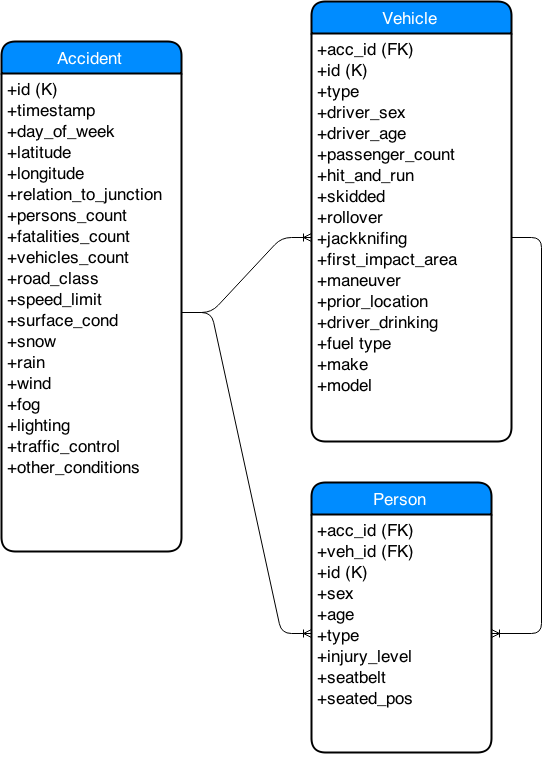
\includegraphics{images/database.png}

\section{Opis tabel}\label{opis-tabel}

\subsection{Accident}\label{accident}

Tabela zawierająca dane i okoliczności dotyczące wypadku

\textbf{Opis pól:}

\begin{itemize}
\item
  id - INT, klucz główny tabeli\\
\item
  timestamp - TIMESTAMP\\
\item
  day\_of\_week - INT, dzień tygodnia\\
\item
  latitude - DECIMAL, szerokość geograficzna - dla USA dane dopiero od
  1999\\
\item
  longtitude - DECIMAL, długość geograficzna - dla USA dane dopiero od
  1999\\
\item
  relation\_to\_junction - STRING

  \begin{itemize}
  \itemsep1pt\parskip0pt\parsep0pt
  \item
    NON\_JUNCTION\\
  \item
    INTERSECTION\\
  \item
    DRIVEWAY - podjazd / prywatna droga\\
  \item
    RAMP - wjazd / zjazd z autostrady\\
  \item
    UNKNOWN\\
  \end{itemize}
\item
  persons\_count - INT, liczba uczestników w wypadku\\
\item
  fatalities\_count - INT, liczba ofiar śmiertelnych wypadku\\
\item
  vehicles\_count - INT, liczba pojazdów biorących udział w wypadku\\
\item
  road\_class - STRING, rodzaj drogi

  \begin{itemize}
  \itemsep1pt\parskip0pt\parsep0pt
  \item
    MOTORWAY - amerykańskie Highway\\
  \item
    PRINCIPAL - brytyjska klasa A, amerykańskie Principal Arterial\\
  \item
    MAJOR - brytyjska B\\
  \item
    MINOR - brytysjka C\\
  \item
    UNCLASSIFIED\\
  \item
    UNKNOWN\\
  \end{itemize}
\item
  speed\_limit - INT, wartość ograniczenia prędkości na drodze
  {[}km/h{]}\\
\item
  surface\_cond - STRING, stan nawierzchni

  \begin{itemize}
  \itemsep1pt\parskip0pt\parsep0pt
  \item
    DRY\\
  \item
    WET\\
  \item
    SNOW\\
  \item
    ICE\\
  \item
    FLOOD\\
  \item
    OTHER (oil, mud, sand, gravel)\\
  \item
    UNKNOWN\\
  \end{itemize}
\item
  snow - STRING, śnieg

  \begin{itemize}
  \itemsep1pt\parskip0pt\parsep0pt
  \item
    YES - dangerous wind conditions\\
  \item
    NO\\
  \item
    UNKNOWN\\
  \end{itemize}
\item
  rain - STRING, deszcz

  \begin{itemize}
  \itemsep1pt\parskip0pt\parsep0pt
  \item
    YES - dangerous wind conditions\\
  \item
    NO\\
  \item
    UNKNOWN\\
  \end{itemize}
\item
  wind - STRING, wiatr

  \begin{itemize}
  \itemsep1pt\parskip0pt\parsep0pt
  \item
    YES - dangerous wind conditions\\
  \item
    NO\\
  \item
    UNKNOWN\\
  \end{itemize}
\item
  fog - mgła

  \begin{itemize}
  \itemsep1pt\parskip0pt\parsep0pt
  \item
    YES - fog, smoke or smog\\
  \item
    NO\\
  \item
    UNKNOWN\\
  \end{itemize}
\item
  lighting - warunki oświetlenia

  \begin{itemize}
  \itemsep1pt\parskip0pt\parsep0pt
  \item
    DAYLIGHT\\
  \item
    DARK\_LIGHTED\\
  \item
    DARK\\
  \item
    UNKNOWN\\
  \end{itemize}
\item
  traffic\_control

  \begin{itemize}
  \itemsep1pt\parskip0pt\parsep0pt
  \item
    TRAFFIC\_SIGNAL\\
  \item
    SIGNAL\_MALF - nie działające światła\\
  \item
    STOP\_SIGN\\
  \item
    AUTH\_PERSON - osoba uprawniona do kierowania ruchem\\
  \item
    NONE - jeżeli wypadek nie na skrzyżowaniu\\
  \item
    UNKNOWN
  \end{itemize}
\end{itemize}

\subsection{Vehicle}\label{vehicle}

Tabela zawierająca dane na temat pojazdów biorących udział w wypadku i
ich kierowców. Jest powiązana relacją n:1 z tabelą \emph{Accident}
poprzez klucz obcy \emph{acc}id\_ - w jednym wypadku może brać udział
wiele pojazdów

\textbf{Opis pól:}

\begin{itemize}
\item
  acc\_id - INT, klucz obcy z tabeli \emph{Accident} realizujący relację
  1:n, wypadek w jakim brał udział dany pojazd\\
\item
  id - INT, klucz główny tabeli\\
\item
  type - STRING

  \begin{itemize}
  \itemsep1pt\parskip0pt\parsep0pt
  \item
    CAR\\
  \item
    MOTORCYCLE\\
  \item
    BUS\\
  \item
    CARGO\\
  \item
    AGRICULTURAL\\
  \item
    OTHER\\
  \item
    UNKNOWN\\
  \end{itemize}
\item
  driver\_sex - STRING, płeć kierowcy

  \begin{itemize}
  \itemsep1pt\parskip0pt\parsep0pt
  \item
    MALE\\
  \item
    FEMALE\\
  \item
    UNKNOWN\\
  \end{itemize}
\item
  driver\_age - INT, wiek kierowcy\\
\item
  passenger\_count - INT, liczba pasażerów\\
\item
  hit\_and\_run - STRING, czy kierujący pojazdem uciekł z miejsca
  wypadku

  \begin{itemize}
  \itemsep1pt\parskip0pt\parsep0pt
  \item
    YES\\
  \item
    NO\\
  \item
    UNKNOWN\\
  \end{itemize}
\item
  skidded - STRING, okoliczności dotyczące poślizgu - dla USA dane te
  występują tylko w latach 2010 - 2013.

  \begin{itemize}
  \itemsep1pt\parskip0pt\parsep0pt
  \item
    YES\\
  \item
    NO\\
  \item
    UNKNOWN\\
  \end{itemize}
\item
  rollover - STRING, okoliczności dotyczące dachowania

  \begin{itemize}
  \itemsep1pt\parskip0pt\parsep0pt
  \item
    YES\\
  \item
    NO\\
  \item
    UNKNOWN\\
  \end{itemize}
\item
  jackknifing - STRING, okoliczności dotyczące jackknifingu

  \begin{itemize}
  \itemsep1pt\parskip0pt\parsep0pt
  \item
    YES\\
  \item
    NO\\
  \item
    UNKNOWN\\
  \end{itemize}
\item
  first\_impact\_area - STRING, pierwsze miejsce uderzenia pojazdu

  \begin{itemize}
  \itemsep1pt\parskip0pt\parsep0pt
  \item
    FRONT\\
  \item
    BACK\\
  \item
    LEFT\_SIDE\\
  \item
    RIGHT\_SIDE\\
  \item
    NON\_COLLISION\\
  \item
    UNKNOWN\\
  \end{itemize}
\item
  maneuver - STRING - dla USA dane te występują tylko w latach 1982 -
  2008.

  \begin{itemize}
  \itemsep1pt\parskip0pt\parsep0pt
  \item
    STRAIGHT\\
  \item
    PARKED\\
  \item
    REVERSING\\
  \item
    U\_TURN\\
  \item
    LEFT\\
  \item
    RIGHT\\
  \item
    CHANGING\_LANE\\
  \item
    OVERTAKING\\
  \item
    HELD\_UP\\
  \item
    STOPPING\\
  \item
    STARTING\\
  \item
    CURVING\\
  \item
    UNKNOWN\\
  \end{itemize}
\item
  driver\_drinking - STRING, obecność alkoholu we krwi kierowcy

  \begin{itemize}
  \itemsep1pt\parskip0pt\parsep0pt
  \item
    YES\\
  \item
    NO\\
  \item
    UNKNOWN\\
  \end{itemize}
\item
  fuel\_type - STRING, rodzaj paliwa - dla USA, do roku 2009, te dane
  zbierane były tylko dla ciężarówek.

  \begin{itemize}
  \itemsep1pt\parskip0pt\parsep0pt
  \item
    DIESEL\\
  \item
    PETROL\\
  \item
    HYBRID\\
  \item
    GAS\\
  \item
    OTHER\\
  \item
    UNKNOWN
  \end{itemize}
\end{itemize}

\subsection{Person}\label{person}

Tabela zawierająca dane na temat uczestników wypadku. Powiązana relacją
n:1 z tabelą \emph{Accident} poprzez klucz obcy \emph{acc}id\_ - w
jednym wypadku może być wiele ofiar. Powiązana relacją n:1..0 z tabelą
\emph{Vehicle} poprzez klucz obcy \emph{veh}id\_ - w jednym pojeździe
może się znajdować wielu uczestników, uczestnik może się znajdować w
jednym pojeździe, lub być pieszym i nie znajdować się w żadnym
pojeździe.

\textbf{Opis pól:}

\begin{itemize}
\item
  acc\_idd - INT, klucz obcy z tabeli \emph{Accident} realizujący
  relację 1:n, wypadek w jakim brał udział dany uczestnik\\
\item
  veh\_id - INT, klucz obcy z tabeli \emph{Vehicle} realizujący relację
  0..1:n, wypadek w jakim brał udział dany uczestnik. Może zawierać
  wartość NULL.\\
\item
  id - INT, klucz główny tabeli\\
\item
  sex - STRING, płeć

  \begin{itemize}
  \itemsep1pt\parskip0pt\parsep0pt
  \item
    MALE\\
  \item
    FEMALE\\
  \item
    UNKNOWN\\
  \end{itemize}
\item
  age - INT, wiek\\
\item
  type - STRING

  \begin{itemize}
  \itemsep1pt\parskip0pt\parsep0pt
  \item
    DRIVER\\
  \item
    PASSENGER\\
  \item
    PEDESTRIAN\\
  \item
    UNKNOWN\\
  \end{itemize}
\item
  injury\_level - STRING, powaga obrażeń

  \begin{itemize}
  \itemsep1pt\parskip0pt\parsep0pt
  \item
    FATAL\\
  \item
    SERIOUS\\
  \item
    SLIGHT\\
  \item
    NONE\\
  \item
    UNKNOWN\\
  \end{itemize}
\item
  seatbelt - STRING, użycie pasów bezpieczeństwa

  \begin{itemize}
  \itemsep1pt\parskip0pt\parsep0pt
  \item
    NOT\_APPLICABLE\\
  \item
    WORN\_CONFIRMED\\
  \item
    WORN\_NOT\_CONFIRMED\\
  \item
    NOT\_WORN\\
  \item
    UNKNOWN\\
  \end{itemize}
\item
  seated\_pos - STRING, miejsce siedzenia w pojeździe

  \begin{itemize}
  \itemsep1pt\parskip0pt\parsep0pt
  \item
    DRIVER\\
  \item
    PASSENGER\\
  \item
    BACK\\
  \item
    NONE\\
  \item
    UNKNOWN
  \end{itemize}
\end{itemize}
